\section{Arreglo de compuertas OR, AND y XOR en VHDL \label{sec:s1}}

\begin{center}
	\begin{minipage}{12cm}
		\begin{tcolorbox}[title=Actividad 1]
			Compilar los dos códigos vistos en clase (VHDL) y observar el resultado con el visor RTL.
		\end{tcolorbox}	
	\end{minipage}
\end{center}

La visualización RTL del arreglo de compuertas OR (primer código), descrito en VHDL, se muestra en la \autoref{fig:forgenerate1_vhdl_rtl}. La implementación se hace instanciando 8 veces al módulo denominado ``MyOr2'' (debido a que las dos entradas son de 8 bits), que simplemente es una compuerta OR de 1 bit (ver \autoref{fig:forgenerate1_vhdl_rtl2}). Las simulaciones se visualizan en la \autoref{fig:forgenerate1_vhdl_wave}, en donde se muestra que este arreglo de compuerta OR opera de manera correcta.

En los Anexos se localiza la descripción en VHDL del primer código. Primeramente se declaran las librerías a utilizar y las señales de entrada y salida. Ahora bien, en la zona declarativa se describe un componente denominado ``MyOr2'', declarando sus entradas y salida. En la zona de la arquitectura, se utiliza a la estructura \textit{for-generate} para instanciar al componente descrito anteriormente. Algunos puntos importantes son que el ciclo \textit{generate} se denomina G0, mientras que las instancias llevan la nomenclatura U0, además, se usa una variable de iteración denominada ``n'' pero no se declara antes de comenzar el ciclo de instancias de hardware. Finalmente, después de declarar la arquitectura del módulo principal, se describe a la entidad ``MyOr2'', declarando nuevamente las librerías a utilizar, las señales de entrada y salida y el comportamiento dentro de la arquitectura.

La visualización RTL del arreglo de compuertas OR, AND y XOR (segundo código), descrito en VHDL, se muestra en la \autoref{fig:forgenerate2_vhdl_rtl}. La implementación se hace nuevamente instanciando 8 veces al módulo denominado ``MyOr2'', no obstante, se agregan 4 instancias de compuertas AND para los 4 bits menos significativos de las entradas A y B, y otras 4 instancias de compuertas XOR para los 4 bits más significativos (ver \autoref{fig:forgenerate2_vhdl_rtl2}). Las simulaciones se visualizan en la \autoref{fig:forgenerate2_vhdl_wave}, en donde se muestra que este arreglo de compuertas OR, AND y XOR opera de manera correcta.

En los Anexos se localiza la descripción en VHDL del segundo código. Así como en el primer código se declaran las librerías a utilizar, las señales de entrada y salida y en la zona declarativa se describe un componente denominado ``MyOr2'', declarando sus entradas y salida. En la zona de la arquitectura, se utilizan 3 estructuras \textit{for-generate} para instanciar al componente descrito anteriormente, junto con las compuertas AND y XOR, según sea el caso. Algunos puntos importantes son que los ciclos \textit{generate} se denominan G1, G2 y G3, las instancias de ``MyOr2'' llevan la nomenclatura U0, se usa una variable de iteración denominada ``n'' (no declarada antes de las iteraciones) y se utilizan dos estructuras \textit{if} para separar a los 4 bits más y menos significativos. Finalmente, después de declarar la arquitectura del módulo principal, se describe a la entidad ``MyOr2'', declarando nuevamente las librerías a utilizar, las señales de entrada y salida y el comportamiento dentro de la arquitectura.

\begin{figure}[ht]
	\centering
	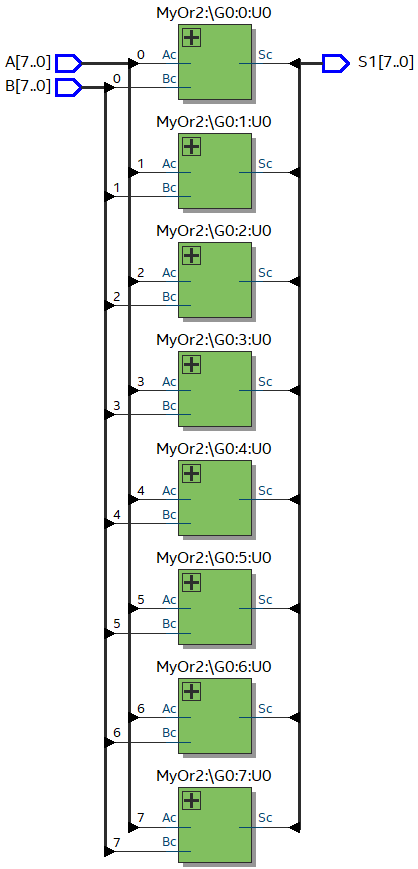
\includegraphics[scale=0.73]{ForGenerate1_VHDL_RTL.png}
	\caption{Diagrama RTL del arreglo de compuertas OR, descrito en VHDL. \label{fig:forgenerate1_vhdl_rtl}}
\end{figure}

\begin{figure}[ht]
	\centering
	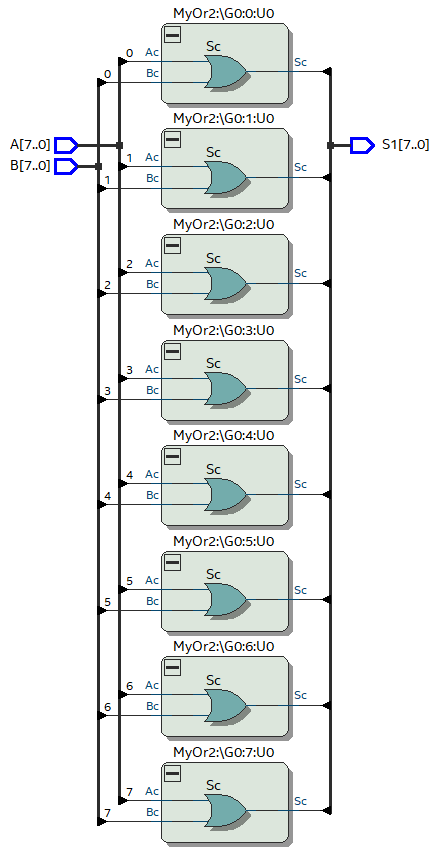
\includegraphics[scale=0.95]{ForGenerate1_VHDL_RTL2.png}
	\caption{Diagrama RTL del arreglo de compuertas OR, descrito en VHDL (vista interna de las instancias). \label{fig:forgenerate1_vhdl_rtl2}}
\end{figure}

\begin{figure}[ht]
	\centering
	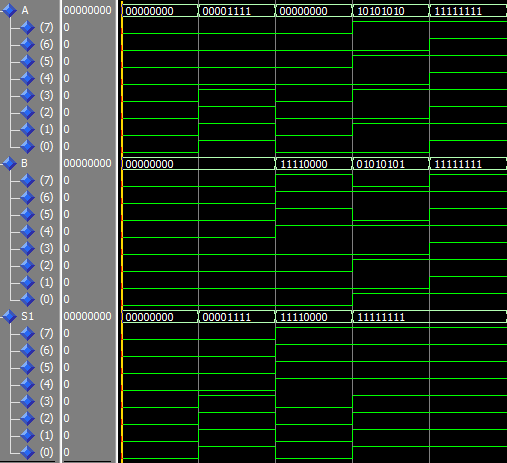
\includegraphics[scale=1.25]{ForGenerate1_VHDL_Wave.png}
	\caption{Simulación del arreglo de compuertas OR, descrito en VHDL, con el visor de formas de onda de ModelSim. \label{fig:forgenerate1_vhdl_wave}}
\end{figure}

\begin{figure}[ht]
	\centering
	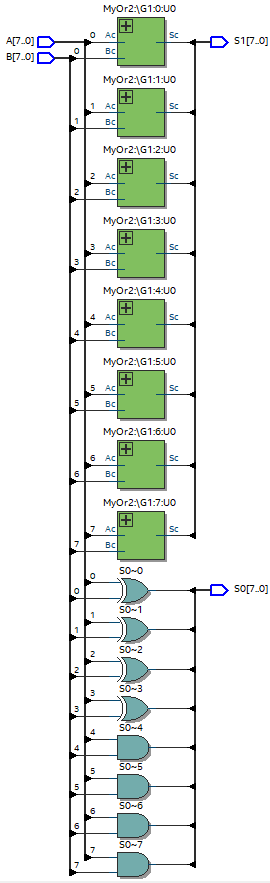
\includegraphics[scale=0.95]{ForGenerate2_VHDL_RTL.png}
	\caption{Diagrama RTL del arreglo de compuertas OR, AND y XOR, descrito en VHDL. \label{fig:forgenerate2_vhdl_rtl}}
\end{figure}

\begin{figure}[ht]
	\centering
	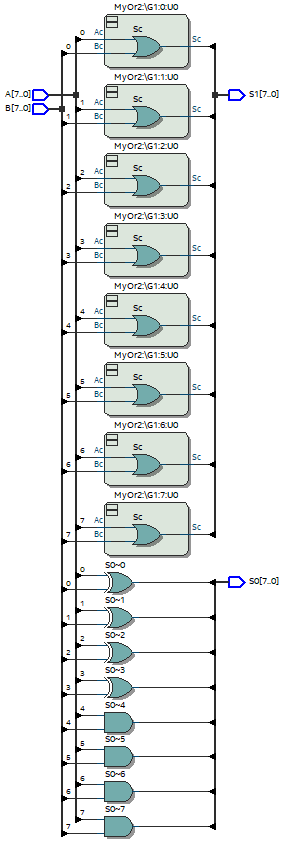
\includegraphics[scale=0.95]{ForGenerate2_VHDL_RTL2.png}
	\caption{Diagrama RTL del arreglo de compuertas OR, AND y XOR, descrito en VHDL (vista interna de las instancias). \label{fig:forgenerate2_vhdl_rtl2}}
\end{figure}

\begin{figure}[ht]
	\centering
	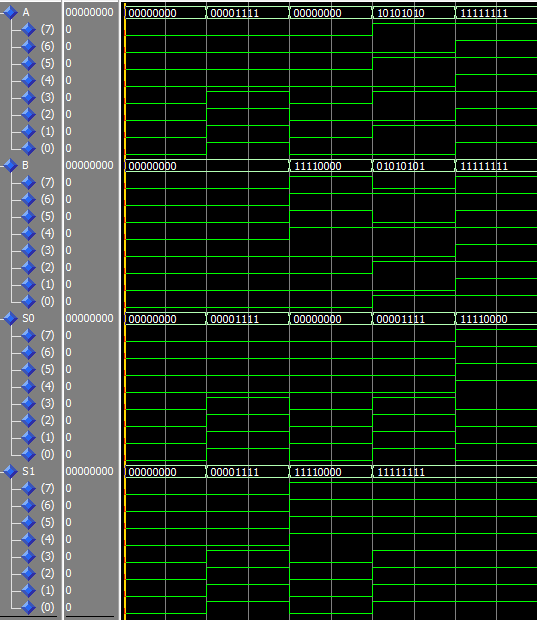
\includegraphics[scale=1.15]{ForGenerate2_VHDL_Wave.png}
	\caption{Simulación del arreglo de compuertas OR, AND y XOR, descrito en VHDL, con el visor de formas de onda de ModelSim. \label{fig:forgenerate2_vhdl_wave}}
\end{figure}